\documentclass[10pt,a4paper]{article}
\usepackage[english]{babel}
\usepackage[utf8]{inputenc}
\usepackage{amsmath, amssymb}
\usepackage{graphicx}
\usepackage{caption}
\usepackage{float}
\usepackage[top=1in, left=1.25in, right=1.25in, bottom=1in]{geometry}
\usepackage[numbered,framed]{matlab-prettifier}
\usepackage{filecontents}
\usepackage[T1]{fontenc}
\usepackage{bigfoot}
\usepackage{listings}

\numberwithin{equation}{subsection}
\newcommand{\eqname}[1]{\tag*{#1}}
\begin{filecontents*}{h21.m}
close all; clear all; clc;
load handel
v = y'/2;
vt=fft(v);
figure(1)
subplot(2,1,1), plot((1:length(v))/Fs,v);
xlabel('Time [sec]'); ylabel('Amplitude');
title('Signal of Interest, v(n)');
set(gca,'Fontsize',12)
% p8 = audioplayer(v, Fs);
% playblocking(p8);

% Set up grid vectors
L=length(v)/Fs;
n=length(v);
t=(1:length(v))/Fs;
k=(2*pi/L)*[0:(n-1)/2 -(n-1)/2:-1]; ks=fftshift(k);

% FFT the unfiltered signal over the entire time domain
subplot(2,1,2), plot(ks/(2*pi),abs(fftshift(vt))/max(abs(vt)))
xlabel('frequency [Hz]'); ylabel('FFT(v(n))');
set(gca,'Fontsize',12)

% Create multiple Gabor filters with (Super) Gaussian, 
% Mexican Hat Wavelet and Shannon window
filter={@(width, t, power) exp(-width*(t).^in), ...
		@(width, t) (1-(t/width).^2).*exp(-((t/width).^2)/2), ...
    	@(width, t) (t>(-width/2) & t<(width/2))};

% Create a sliding window for Gabor transform
vgt_spec=[];
width=1; % window width
dt=0.1; % translation
tslide=0:dt:L;
figure(2)
for j=1:length(tslide)
    g=filter{3}(width, t-tslide(j));
    vg=g.*v; vgt=fft(vg);
    vgt_spec=[vgt_spec; abs(fftshift(vgt))];
    subplot(3,1,1), plot(t,v,'k',t,g,'g')
    ylabel('v(n), g(t)'); xlabel('time [sec]');
    set(gca,'Fontsize',12)
    subplot(3,1,2), plot(t,vg,'k')
    ylabel('v(n)*g(t)'); xlabel('time [sec]');
    set(gca,'Fontsize',12)
    subplot(3,1,3), plot(ks/(2*pi),abs(fftshift(vgt))/max(abs(vgt)))
    ylabel('FFT(vg)'); xlabel('frequency [Hz]');
    set(gca,'Fontsize',12)
    drawnow
    pause(0.1)
end

% Plot the spectrogram
figure(3)
pcolor(tslide,ks/(2*pi),vgt_spec.'), shading interp
ylabel('frequency [Hz]'); xlabel('time [sec]');
set(gca, 'Ylim', [-2000 2000], 'Fontsize', 12)
colormap hot
\end{filecontents*}

\begin{filecontents*}{h22.m}
close all; clear all; clc;
% Set up grid vectors
v=y'/2;
L=length(v)/Fs;
n=length(v);
t=(1:length(v))/Fs;
k=(2*pi/L)*[0:(n/2)-1 -n/2:-1]; ks=fftshift(k);

% Plot signal
figure(1)
% tr_piano=16; % record time in seconds
% y=audioread('music1.wav'); Fs=length(y)/tr_piano;
% plot((1:length(y))/Fs,y);
% xlabel('Time [sec]'); ylabel('Amplitude');
% set(gca, 'Fontsize', 12)
% title('(a) Mary had a little lamb (piano)'); drawnow
tr_rec=14; % record time in seconds
y=audioread('music2.wav'); Fs=length(y)/tr_rec;
plot((1:length(y))/Fs,y);
xlabel('Time [sec]'); ylabel('Amplitude');
title('(a) Mary had a little lamb (recorder)');
% p8 = audioplayer(y,Fs); playblocking(p8);

% Create a siliding window for Gabor transform
vgt_spec=[];
width=1000;
dt=0.14;
tslide=0:dt:L;
for j=1:length(tslide)
    g=exp(-width*(t-tslide(j)).^2); % Gaussian window
    vg=g.*v; vgt=fft(vg);
    vgt_spec=[vgt_spec; abs(fftshift(vgt))];
%     subplot(3,1,1), plot(t,v,'k',t,g,'g')
%     ylabel('v(n), g(t)'); xlabel('time [sec]');
%     set(gca,'Fontsize',12)
%     subplot(3,1,2), plot(t,vg,'k')
%     ylabel('v(n)*g(t)'); xlabel('time [sec]');
%     set(gca,'Fontsize',12)
%     subplot(3,1,3), plot(ks/(2*pi),abs(fftshift(vgt))/max(abs(vgt)))
%     ylabel('FFT(vg)'); xlabel('frequency [Hz]');
%     set(gca,'Fontsize',12)
%     drawnow
%     pause(0.1)
end

% Plot Spectrogram of frequency notes from piano/recorder
figure(2)
pcolor(tslide,ks/(2*pi), vgt_spec.'), shading interp
xlabel('time [sec]'); ylabel('frequency [Hz]'); 
title(sprintf('(b) Spectrogram of Recorder (width=%d, dt=%.2f)', width, dt))
set(gca,'Ylim', [700 1200], 'Fontsize', 12)
colormap hot
\end{filecontents*}

\let\ph\mlplaceholder % shorter macro
\lstMakeShortInline"
\lstset{
  style              = Matlab-editor,
  basicstyle         = \mlttfamily,
  escapechar         = ",
  mlshowsectionrules = true,
}

\title{Amath 482 Winter 2019 \\
HW2: G\'abor transforms}
\author{Wenrui Yuan}
\date{\today}

\begin{document}
\maketitle

\begin{abstract}
	This report performs time frequency analysis on three different audio signals using spectrogram and G\'abor transform. We construct a sliding window filter with varying window width to understand relation between time and frequency resolution. The effect of translational parameter is also considered to explore the idea of undersmapling and oversampling. Moreover, various time filters are constructed to study characteristics of each filter. Finally, we use spectrograms to reproduce music score and the effect of overtones is also concluded.
\end{abstract}


\section{Introduction and Overview}
	In time frequency analysis of a audio signal, we must have knowledge of its components in both time and space domain. However, the Fourier transform fails to accomplish that as it loses all information of time after transform. Therefore, we need a transform that retains both time and frequency information, namely, the G\'abor transform to commence the analysis.\\
	In particular, this reports examines three pieces of audio signals and their spectrograms. We will start with the Handel's piece to understand the correlation of the G\'abor transform and spectrogram. The effect of scaling and translation parameters of the window and different window functions on the corresponding spectrogram will be tested first. We then apply the same idea to the other two pieces of 'Mary had a little lamb' to obtain spectrograms with strong frequencies that can be mapped into music notes for reproducing music scores.


\section{Theoretical Background}
\subsection{Spectrogram}
A spectrogram is very powerful in visualizing varying frequencies on a given time interval. It is especially helpful when analyzing an audio signal as we are interested in both frequency and its associated time information. It also tells the amount of information (or the level of resolution) for each axis, and thus it can helps us to understand characteristics and drawbacks of G\'abor Transform as performed later in this report.

\subsection{G\'abor Transform}
Unlike FFT which loses all temporal information, the G\'abor transform transfers local information of time to the frequency domain so that we have both time and frequency resolution that can help us to locate not only the magnitude of frequency but also its position in the time domain.\\
Generally, a G\'abor Transform, or STFT, has the form \cite{582},
\begin{equation}
\mathcal{G}[f](t,\omega) = \int_{-\infty}^{\infty}f(\tau)\bar{g}(\tau - t)e^{-i\omega\tau}d\tau
\end{equation}
which localize the signal with specified window around $t=\tau$.\\
As one of the windowed Fourier transforms, the G\'abor transform allows us to adjust window size with width and translation parameters. Moreover, there are many window functions of various shapes which can be applied to the transform such as
\begin{align}
g(t) &= e^{-a(t-b)^2} \\ \eqname{Gaussian Function \cite{582}}\\
g(t) &= e^{-a(t-b)^{10}} \\ \eqname{Super Gaussian Function \cite{582}}\\
g(t) &= (1-(\frac{(t-b)}{a})^2)e^{\frac{(t-b)^2}{2a^2}} \\ \eqname{Mexican Hat Wavelet \cite{mhw}}\\
g(t) &= \begin{cases}
0\qquad |t-b| > \frac{1}{2}\\
1\qquad |t-b|\leq\frac{1}{2}
\end{cases}\\ \eqname{Step Function \cite{582}}
\end{align}
where $a$ and $b$ are width and translation parameters respectively. In particular, the Mexican Hat Wavelet is derived from the second order derivative of the Gaussian function with the form $g(t) = e^{-\frac{(t-b)^2}{2a^2}}$. However, the G\'abor transform also has many limitations and the most important one is that there is a trade-off in time and frequency resolution, which means finer time resolution will result in courser frequency resolution and vice versa.


\section{Algorithm Implementation and Development}
Since both parts of this report follow the same principle in applying G\'abor transform, unless specified, this section will cover general steps of implementation for both parts.
\begin{itemize}

\item \textbf{Load and read audio data}\\
We start with loading audio data from Matlab, \texttt{music1.wav} and \texttt{music2.wav}. We're given signal \texttt{Y} and the sampling rate \texttt{Fs} for the first piece and obtain these two for the rest through \texttt{audioread}.

\item \textbf{Set up grid vectors}\\
We then define grid vectors for frequency component \texttt{k}, which needs to be factored by $\frac{2\pi}{L}$ since FFT assumes the $2\pi$ periodic signals. Therefore, it must be shifted back to its mathematically
correct position using \texttt{fftshift} as FFT will results in shifts
of the domain that $[-L, 0] \rightarrow [0, -L]$ and $[0, L] \rightarrow [L, 0]$. \cite{582}

\item \textbf{Construct G\'abor filter with various window functions (Only for Part I)}\\
Define a list of functions with first one being Gaussian and Super Gaussian functions. The second one is the Mexican Hat Wavelet function and the third one is the step function constructed with \texttt{boolean} logic. We only need the Gaussian filter in Part II for its time-efficiency.

\item \textbf{Create a sliding window to perform G\'abor transform}\\
Set \texttt{width} and time steps \texttt{dt} for sliding window \texttt{tslide} and an empty list \texttt{vgt\_spec} for storing spectrum of each slide. Note that \texttt{dt} is fixed but \texttt{tslide} is constantly varying for the window to slide, and thus \texttt{dt} can be seen as the translation parameter. Next, start the loop to apply filters to the signal and FFT it for each time slide. Then we store the filtered, transformed and shifted data into \texttt{vgt\_spec}.

\item \textbf{Plot the signal for each time slide (Only for Part I)}\\
This plot intuitively visualizes the original signal with one of the window functions, their products and its FFT. Note that as FFT assumes the $2\pi$ period, we need to divide \texttt{ks} by $2\pi$ to get the actual frequency representation in Hz unit. As we no more exploring the effect of window width, translations as well as filter functions in part II, this plot is only for part I.

\item \textbf{Plot Spectrograms for the signal}\\
After computing the entire list of spectrum information for the signal, we plot the spectrogram for the signal once a time to explore how each parameters effects the result. Also note that \texttt{ks} has to be divided by $2\pi$ here.

\item \textbf{Read frequency values and find corresponding music notes (Only for Part II)}\\
We map frequencies (in Hz) to the music notes and connect these notes to reproduce music scores for both pieces. We next compare the music score for each pieces with their original one to conclude the effect of overtones.

\end{itemize}


\section{Computational Results}
\subsection*{Part I: Handel's Messiah}
\begin{figure}[H]
\begin{center}
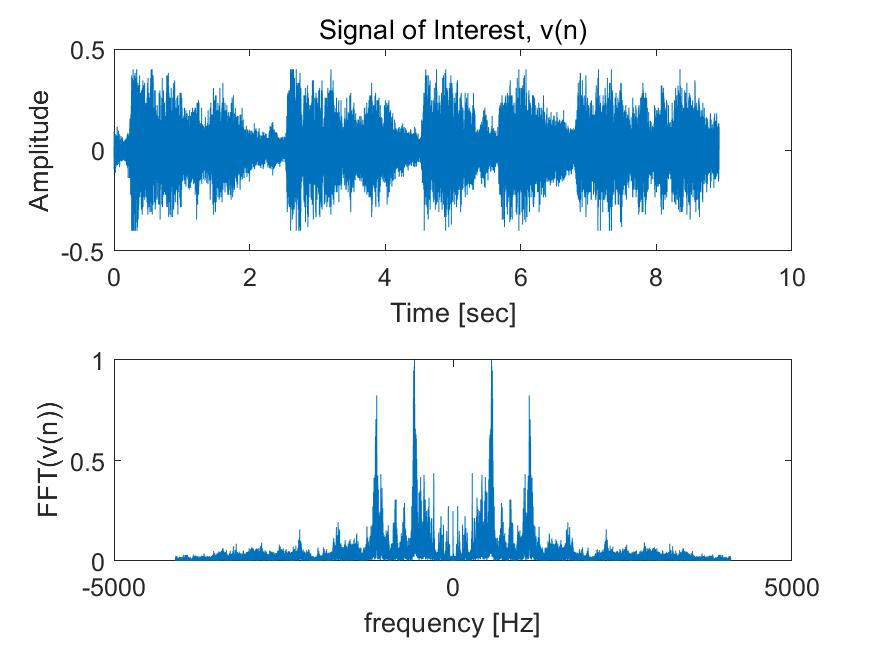
\includegraphics[scale=0.3]{f1.jpg}
\caption{Plot of unfilterd Handel's Messiah signal and its FFT}
\end{center}
\end{figure}

Figure 1 shows the signal of the piece of Handel's Messiah and FFT. However, FFT over the entire time domain is not ideal for signal analysis and the use of G\'abor filtering is therefore necessary.

\begin{figure}[H]
\begin{center}
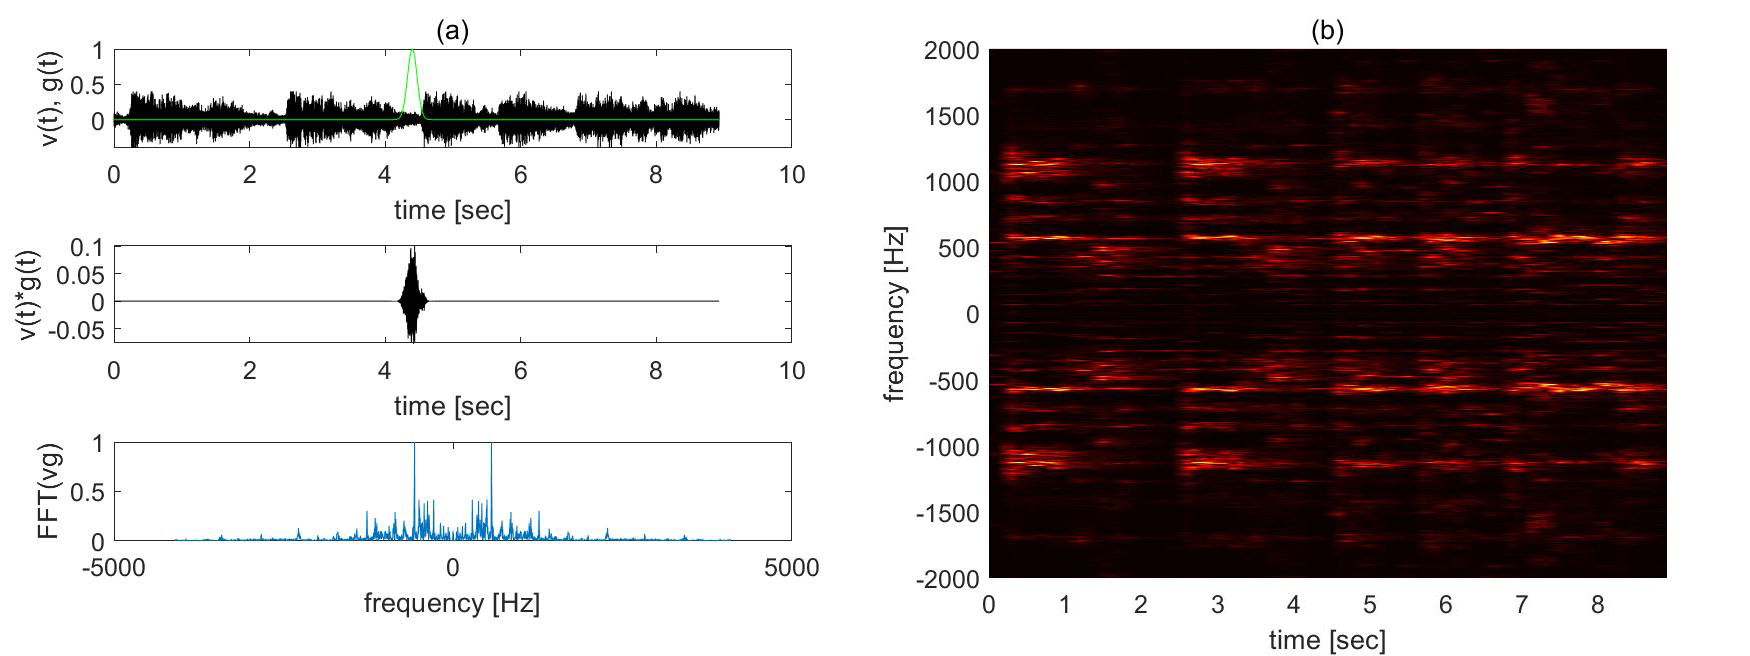
\includegraphics[scale=0.22]{f2.jpg}
\caption{Plot and spectrogram of Handel's Messiah signal with G\'abor filter using Gaussian window \texttt{(width = 1, $\Delta t$ = 0.1)}}
\end{center}
\end{figure}

We start with Gaussian window of width 100 as shown in the top of Figure 2(a). The one in the middle represents signal within the window(i.e. filtered signal) and the bottom one shows FFT of filtered signal. Figure 2(b) is the corresponding spectrogram.

\begin{figure}[H]
\begin{center}
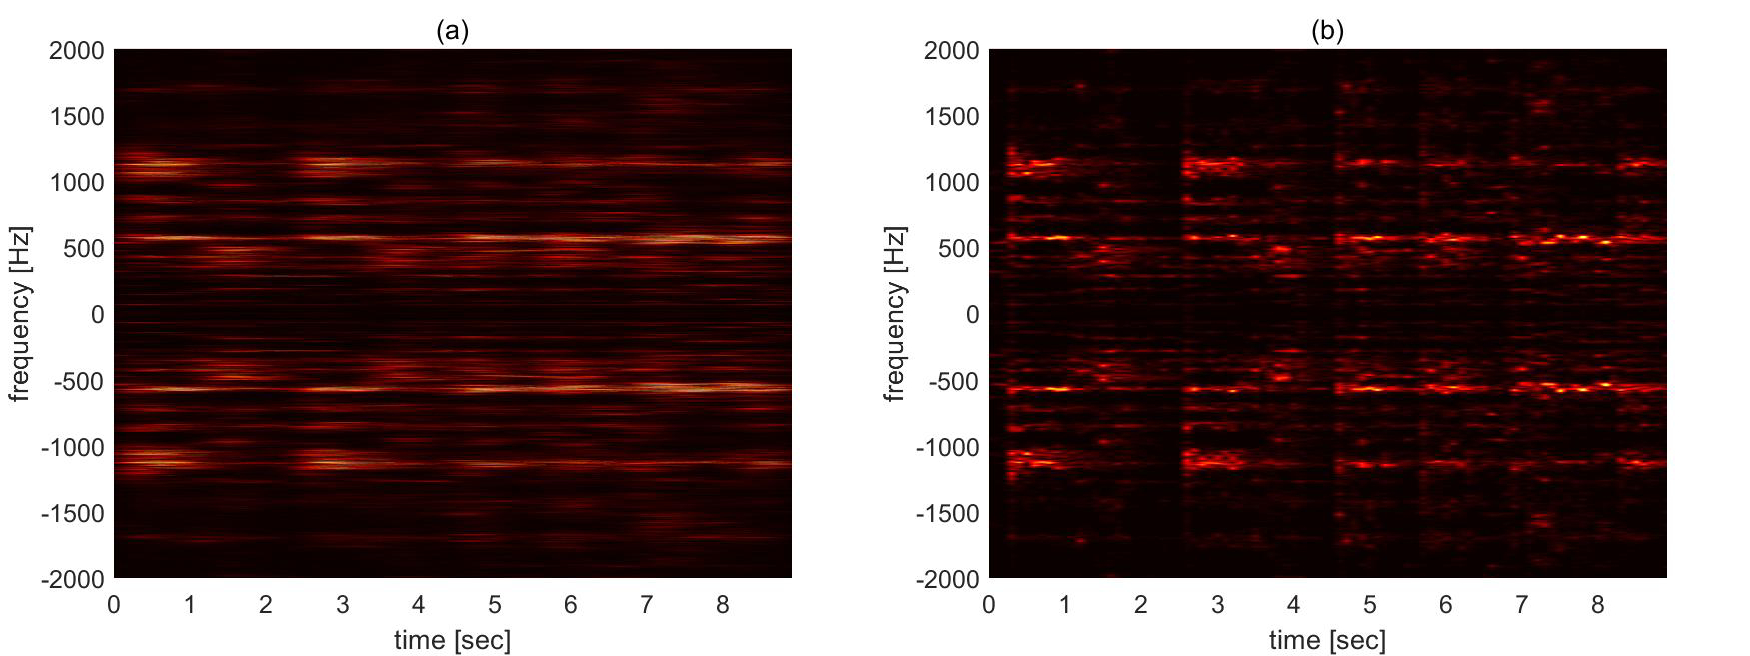
\includegraphics[scale=0.22]{f3.jpg}
\caption{Spectrogram of Handel signal after G\'abor filtering using Gaussian window of (a) \texttt{width = 10 } and (b) \texttt{width = 1000}}
\end{center}
\end{figure}

Next, we explore how window width effects spectrogram. In particular, as window gets narrower(width value increases), we achieved better time resolution at the cost of losing frequency resolution.

\begin{figure}[H]
\begin{center}
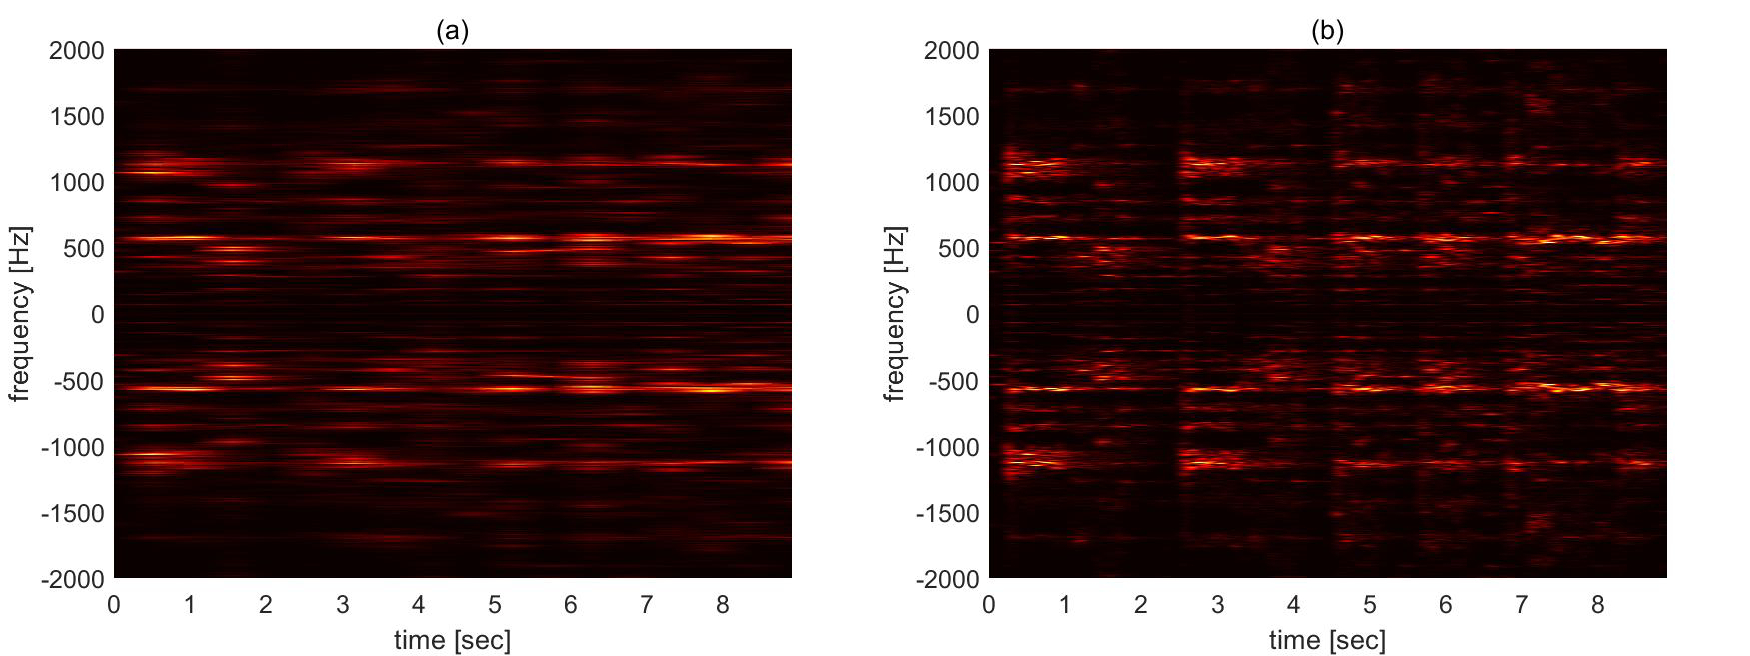
\includegraphics[scale=0.22]{f4.jpg}
\caption{Spectrogram of Handel signal after G\'abor filtering using Gaussian window(width = 100) and different translation values (a)$\Delta t = 0.5s$ (undersampling) and (b) $\Delta t = 0.01s$ (oversampling)}
\end{center}
\end{figure}

Figure 4 presents spectrogram with different translation values which can be seen as the sampling rate. Clearly 4(a)'s frequency component is washed out due to the 0.5s time step and= there are not enough samples (signal) to describe the frequency. On the other hand, 4(b) is much finer but not time-efficient as it takes too much samples, with many of them being unnecessary.

\begin{figure}[H]
\begin{center}
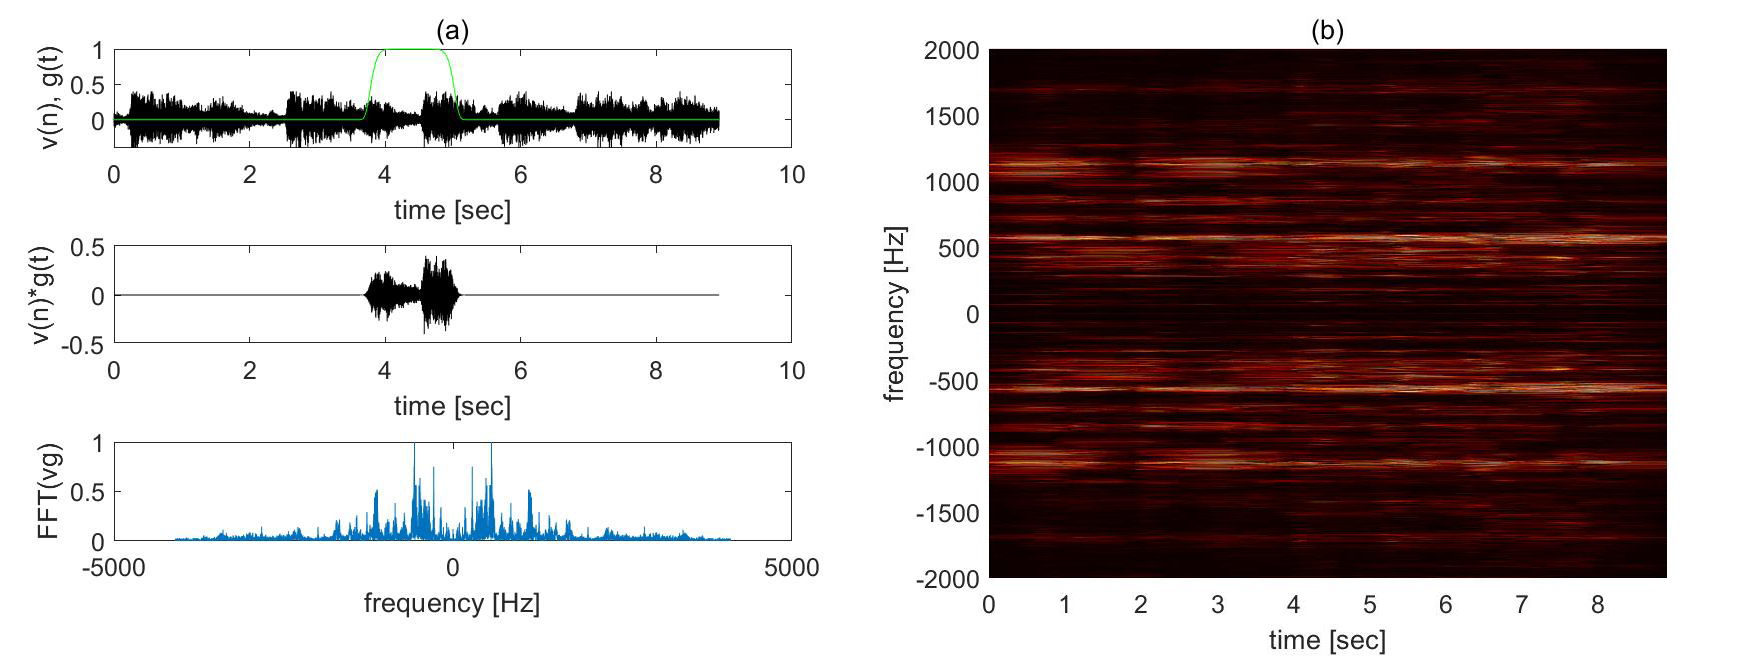
\includegraphics[scale=0.22]{f5.jpg}
\caption{Plot and spectrogram of Handel signal after G\'abor filtering using Super Gaussian window \texttt{(width = 100, $\Delta t$ = 0.1)}}
\end{center}
\end{figure}

\begin{figure}[H]
\begin{center}
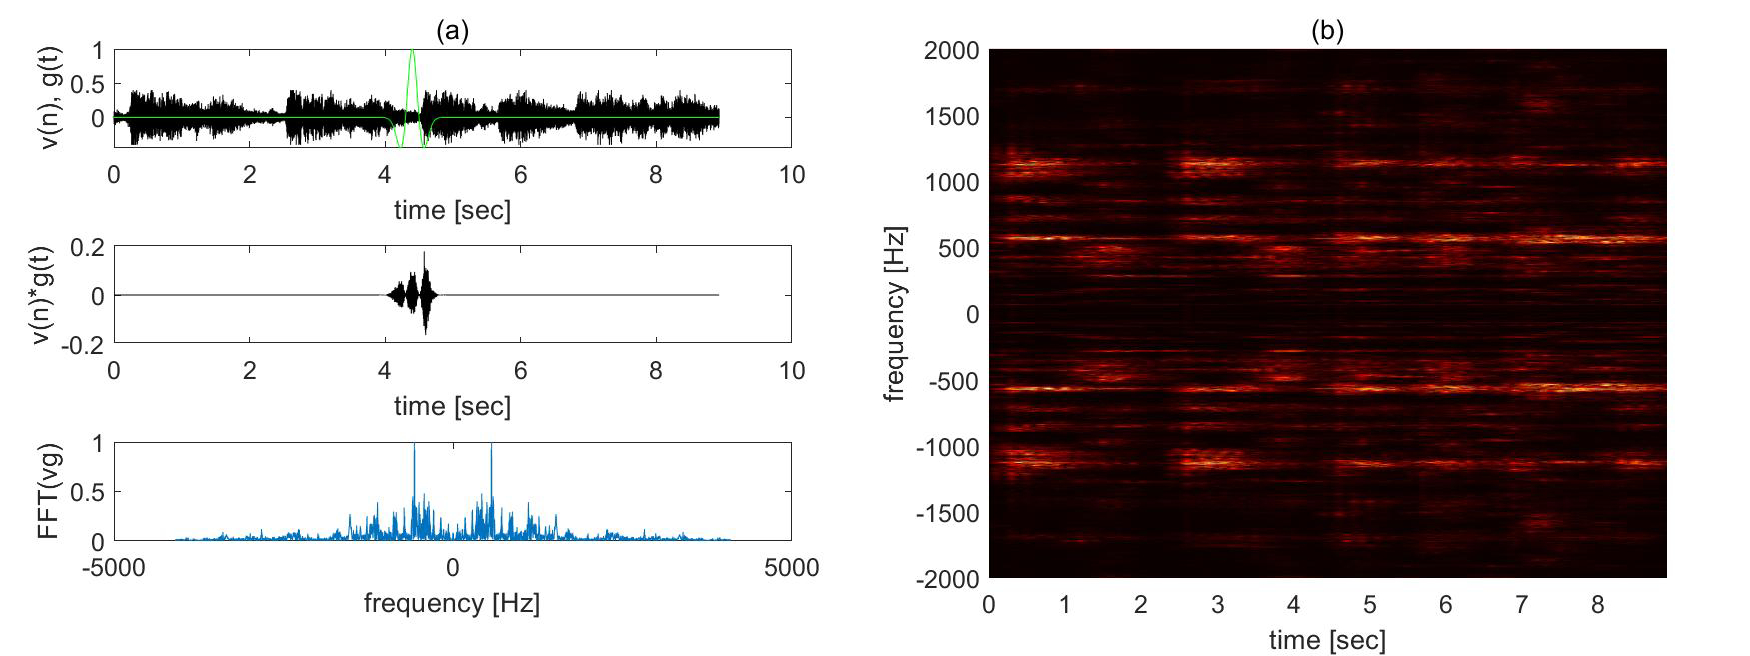
\includegraphics[scale=0.22]{f6.jpg}
\caption{Plot and spectrogram of Handel signal after G\'abor filtering using Mexican Hat Wavelet window \texttt{(width = 0.1, $\Delta t$ = 0.1)}}
\end{center}
\end{figure}
	
\begin{figure}[H]
\begin{center}
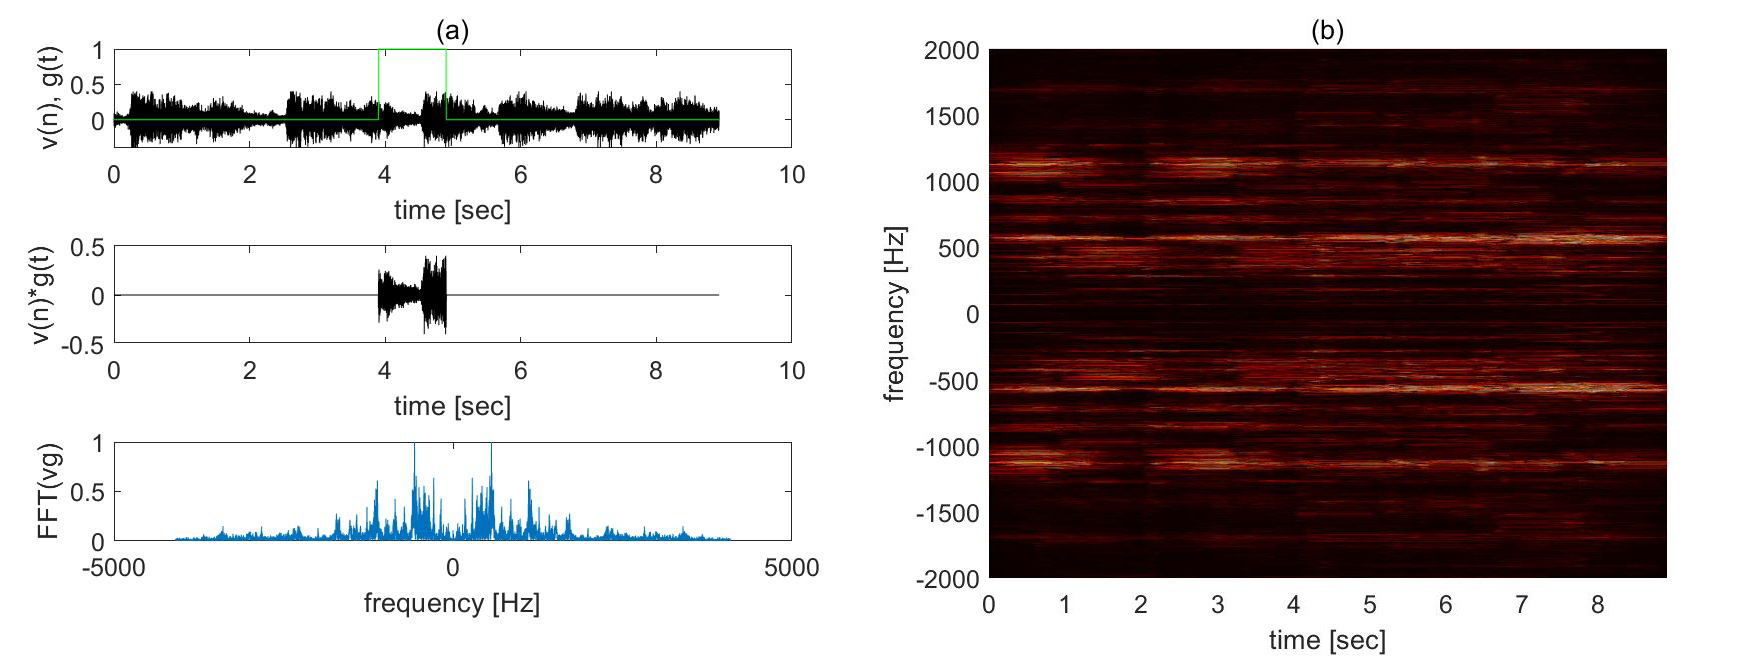
\includegraphics[scale=0.22]{f7.jpg}
\caption{Spectrogram of Handel signal after G\'abor filtering using Shannon window\\ \texttt{(width = 1, $\Delta t$ = 0.1)}}
\end{center}
\end{figure}
	
We then explore spectrograms with different window functions(Super Gaussian, Mexican Hat Wavelet, Shannon) shown in figure 5, 6 and 7. As the shape of Mexican Hat Wavelet and Gaussian function resemble, they share similar spectrograms with better time resolution but worse frequency one. Same principle applies to Shannon and Super Gaussian function as well while their spectrograms have better frequency resolution but worse time resolution.

\subsection*{Part II: Marry had a little lamb}
\begin{figure}[H]
\begin{center}
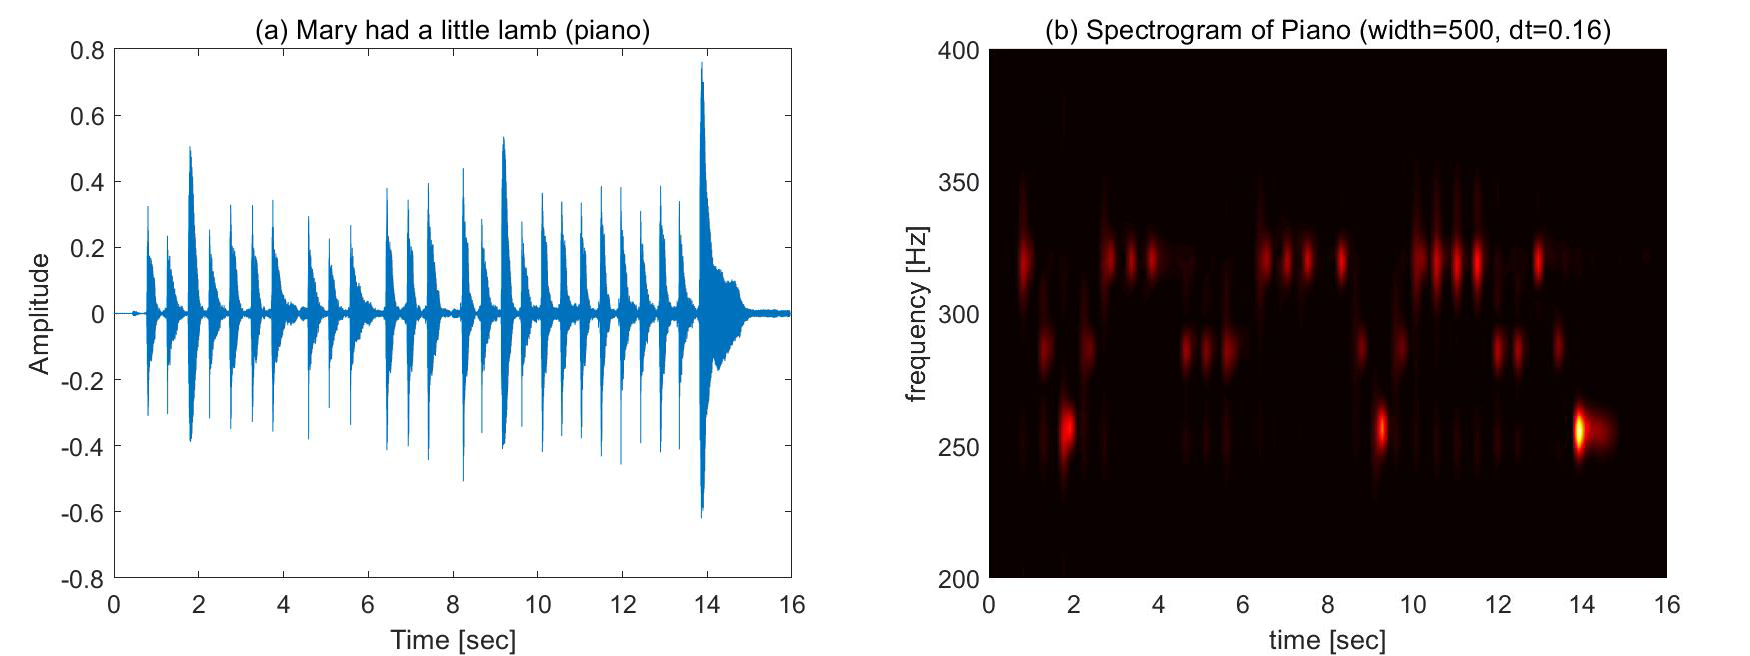
\includegraphics[scale=0.22]{f8.jpg}
\caption{Spectrogram of piano signal after G\'abor filtering using Gaussian window\\ \texttt{(width = 500, $\Delta t$ = 0.16)}}
\end{center}
\end{figure}
	
Figure 8 gives us frequency of piano signal. We then map each frequency (in Hz) to the nearest music note and thus the music score for this piece is $E_4-D_4-C_4-D_4-E_4-E_4-E_4-D_4-D_4-D_4-E_4-E_4-E_4 \quad E_4-D_4-C_4-E_4-E_4-E_4-E_4-D_4-D_4-E_4-D_4-C_4$, which is exactly how the original piece sounds like.
	
\begin{figure}[H]
\begin{center}
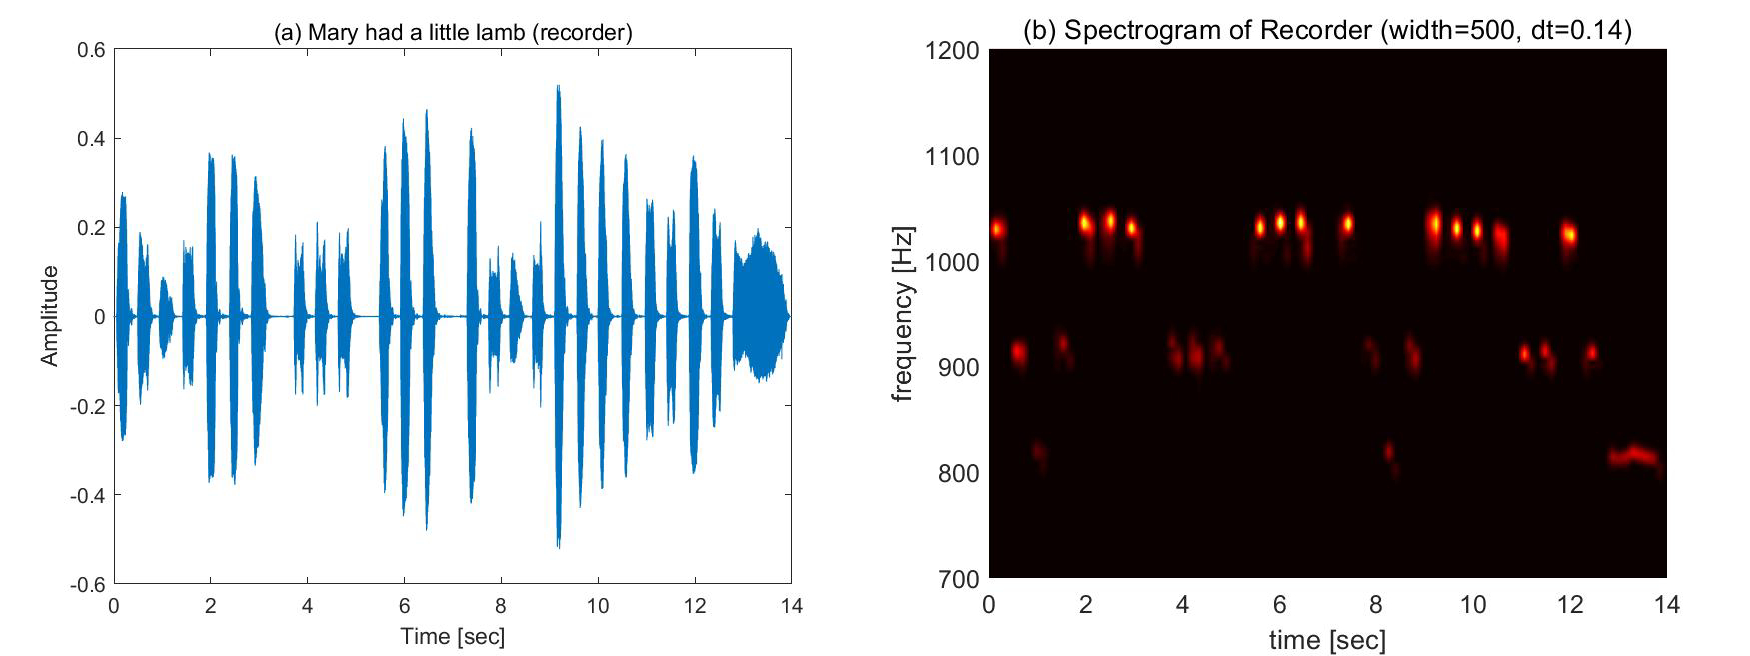
\includegraphics[scale=0.22]{f9.jpg}
\caption{Spectrogram of recorder signal after G\'abor filtering using Gaussian window\\ \texttt{(width = 500, $\Delta t$ = 0.14)}}
\end{center}
\end{figure}
	
Similarly, the music score derived from frequencies in figure 9(b) is $C_6-B_5-A_5-B_5-C_6-C_6-C_6-B_5-B_5-B_5-C_6-C_6-C_6 \quad C_6-B_5-A_5-B_5-C_6-C_6-C_6-C_6-B_5-B_5-C_6-B_4-A_5$, which has a slight deviation in keys but noticeable distortion in signal compared with the original piece. Compared with the piano signal, it is obvious that signal from recorder has more overtones around each central frequency and thus the corresponding spectrogram is less accurate.


\section{Summary and Conclusions}
In part I, We understand how can we perform time-frequency analysis without loosing time resolution through G\'abor transform. In particular, we learned that time and frequency resolutions are trade-offs in G\'abor transform by adjusting window width and time step(translations). Merits and drawbacks of each window function are also studied by comparing their spectrograms.\\
While in part II, we compared signals from piano and recorder of the same piece of work and reproduced music scores from spectrograms of each file. We noticed that the reproduced music score for recorder differs from the original piece of work vastly, which is possibly caused by overtones generated from the instrument.


\begin{thebibliography}{11}
	\bibitem{582}
	J. Nathan Kutz. 2013.
	\textit{Data-Driven Modeling \& Scientific Computation}. p. 53-74
	
	\bibitem{mtlb}
	\textit{Matlab Documentation. Mathworks}; [2019 Feb 11]. \\https://www.mathworks.com/help/index.html

	\bibitem{mhw}
	\textit{Mexican Hat Wavelet. Wikipedia}; [2019 Feb 12]. \\https://www.en.wikipedia.org/wiki/Mexican\_Hat\_Wavelet	
\end{thebibliography}


\section*{Appendix A: MATLAB functions used}
	\begin{itemize}
		\item \texttt{audioplayer}\\
		\texttt{audioplayer(Y, Fs)} creates an audioplayer for signal \texttt{Y} with a sample rate \texttt{Fs}
		\item \texttt{playblocking}\\
		Play the audio file in \texttt{audioplayer}
		\item \texttt{fft}\\
		Computes the 1-D Fourier transform using FFT algorithm
		\item \texttt{fftshift}\\
		Shifts zero-frequency to the center
		\item \texttt{pcolor}\\
		\texttt{pcolor(X, Y, C)} draws a pseudocolor plot for \texttt{C} with grid vectors \texttt{X} and \texttt{Y}.
		\item \texttt{audioread}\\
		Reads data from specified file and returns a signal \texttt{Y} and 	sampling rate \texttt{Fs}.
	\end{itemize}


\section*{Appendix B: MATLAB codes}
\subsection*{Part I: Handel's Messiah}
\lstinputlisting{h21.m}

\subsection*{Part II: Marry had a little lamb}
\lstinputlisting{h22.m}


\end{document}
